%=====================================================================
%  MMSS Graph Theory : Daily Report + Solutions
%
%  This is the only file you edit day to day.
%  All packages, styles and graph macros live in backend.tex.
%  Cheat sheet for the graph toolkit: top of backend.tex, or readme.txt.
%=====================================================================
\documentclass[11pt]{article}

%settings
\newcommand{\teamname}{[GROUP NAME]}
\newcommand{\reportdate}{\today}
\newcommand{\logopath}{assets/logo.png}  


%=====================================================================
%  backend.tex : MMSS Graph Theory report engine
%
%  DO NOT edit this file for day-to-day reports. Edit main.tex.
%  Touch this file only when you want a NEW macro or a style change.
%  (Makers note : This was really hard to make and I strongly suggest 
%  you dont touch it T-T....)
%  Loaded by main.tex via %=====================================================================
%  backend.tex : MMSS Graph Theory report engine
%
%  DO NOT edit this file for day-to-day reports. Edit main.tex.
%  Touch this file only when you want a NEW macro or a style change.
%  (Makers note : This was really hard to make and I strongly suggest 
%  you dont touch it T-T....)
%  Loaded by main.tex via %=====================================================================
%  backend.tex : MMSS Graph Theory report engine
%
%  DO NOT edit this file for day-to-day reports. Edit main.tex.
%  Touch this file only when you want a NEW macro or a style change.
%  (Makers note : This was really hard to make and I strongly suggest 
%  you dont touch it T-T....)
%  Loaded by main.tex via \input{backend} (after \documentclass).
%
%  Expects (optionally) these to be defined in main.tex BEFORE \input:
%    \teamname    \reportdate    \logopath
%  Fallbacks are provided below, so nothing breaks if you forget.
%
%  ---------------------------------------------------------------
%  GRAPH TOOLKIT CHEAT SHEET  (all calls go INSIDE graphfig/tikzpicture)
%  ---------------------------------------------------------------
%    \gcycle{n}{radius}{prefix}      n vertices on a circle, joined as a cycle
%    \gcyclen{n}{radius}{prefix}     same, vertices labelled 1..n
%    \gcomplete{n}{radius}{prefix}   complete graph K_n on a circle
%    \gbipartite{m}{n}{gap}          complete bipartite K_{m,n}
%                                      handles: left bl1..blm, right br1..brn
%    \gpath{n}{spacing}{prefix}      path on n vertices, left to right
%    \gpetersen                      Petersen graph  (\gpeterson kept as alias)
%                                      handles: outer po0..po4, inner pin0..pin4
%    \gcube{n}                       n x n x n grid cube, oblique 2D projection
%    \gqgon{n}, \gpancake{n}         suprise hidden functions, only use after you 
%                                      learned what it is. 
%
%  Named handles stay live for the rest of the picture, so after a call:
%    \draw[edge,densely dashed] (po0)--(pin2);   or   \node[hv] at (bl1){};
%
%  Vertex styles:  v (filled dot) . ov (open ring) . hv (highlighted hub)
%  Edge style:     edge
%
%  Figure wrapper: \begin{graphfig}[scale]{Label} ... \end{graphfig}
%    {Text} -> centred, titled  [Graph Text]
%    {NUM}  -> centred, auto-numbered  [Graph 1], [Graph 2], ...
%    {}     -> bare, no title, no centring (use to line pictures up side by side)
%=====================================================================

\usepackage[margin=1in,headheight=30pt,headsep=16pt]{geometry}
\usepackage{amsmath,amssymb,amsfonts,amsthm}
\usepackage{enumitem}
\usepackage{fancyhdr}
\usepackage{graphicx}
\usepackage{tikz}
\usepackage{xcolor}
\usetikzlibrary{arrows.meta,calc}


\providecommand{\teamname}{[GROUP NAME]}
\providecommand{\reportdate}{\today}
\providecommand{\logopath}{assets/logo.png}

\pagestyle{fancy}
\fancyhf{}
\renewcommand{\headrulewidth}{0.4pt}
\renewcommand{\footrulewidth}{0pt}
\fancyhead[L]{\raisebox{2pt}{\small\textsc{\teamname}}}
\fancyhead[R]{\expandafter\IfFileExists\expandafter{\logopath}
  {\includegraphics[height=10pt]{\logopath}}{}}
\fancyfoot[C]{\small\thepage}

\fancypagestyle{firstpage}{
  \fancyhf{}
  \renewcommand{\headrulewidth}{0pt}
  \fancyfoot[C]{\small\thepage}
}

\setlength{\parindent}{0pt}
\setlength{\parskip}{6pt}

\newcommand{\divider}{\begin{center}\rule{0.6\textwidth}{0.4pt}\end{center}}

\newtheoremstyle{solstyle}{6pt}{6pt}{}{}{\bfseries}{.}{ }{}
\theoremstyle{solstyle}
\newtheorem*{solution}{Solution}

\newcommand{\WLoG}{WLoG}
\newcommand{\Cn}[1]{C_{#1}}
\newcommand{\Kn}[1]{K_{#1}}
\newcommand{\Kt}[2]{K_{#1,#2}}

\tikzset{
  v/.style ={circle, fill=black, inner sep=1.6pt},
  ov/.style={circle, draw=black, fill=white, line width=0.6pt, inner sep=1.6pt},
  hv/.style={circle, fill=black!55, draw=black, line width=0.6pt, inner sep=2.6pt},
  edge/.style={line width=0.6pt},
}


\newcommand{\gcycle}[3]{
  \foreach \gi in {1,...,#1}{\node[v] (#3\gi) at ({90-(\gi-1)*360/#1}:#2){};}
  \foreach \gi in {1,...,#1}{\pgfmathtruncatemacro{\gj}{mod(\gi,#1)+1}\draw[edge] (#3\gi)--(#3\gj);}
}

\newcommand{\gcyclen}[3]{
  \foreach \gi in {1,...,#1}{
    \pgfmathsetmacro{\gang}{90-(\gi-1)*360/#1}
    \node[v,label={\gang:\gi}] (#3\gi) at (\gang:#2){};}
  \foreach \gi in {1,...,#1}{\pgfmathtruncatemacro{\gj}{mod(\gi,#1)+1}\draw[edge] (#3\gi)--(#3\gj);}
}

\newcommand{\gcomplete}[3]{
  \foreach \gi in {1,...,#1}{\node[v] (#3\gi) at ({90-(\gi-1)*360/#1}:#2){};}
  \foreach \gi in {1,...,#1}{\foreach \gj in {1,...,#1}{\ifnum\gi<\gj\relax\draw[edge] (#3\gi)--(#3\gj);\fi}}
}

\newcommand{\gbipartite}[3]{
  \foreach \gi in {1,...,#1}{\node[v] (bl\gi) at (0,{(#1+1)/2-\gi}){};}
  \foreach \gj in {1,...,#2}{\node[v] (br\gj) at (#3,{(#2+1)/2-\gj}){};}
  \foreach \gi in {1,...,#1}{\foreach \gj in {1,...,#2}{\draw[edge] (bl\gi)--(br\gj);}}
}

\newcommand{\gpath}[3]{
  \foreach \gi in {1,...,#1}{\node[v] (#3\gi) at ({(\gi-1)*#2},0){};}
  \pgfmathtruncatemacro{\gplast}{#1-1}
  \foreach \gi in {1,...,\gplast}{\pgfmathtruncatemacro{\gpk}{\gi+1}\draw[edge] (#3\gi)--(#3\gpk);}
}


\newcommand{\gpetersen}{
  \foreach \gp in {0,...,4}{
    \node[v] (po\gp) at ({90+\gp*72}:2){};
    \node[v] (pin\gp) at ({90+\gp*72}:1){};}
  \foreach \gp in {0,...,4}{
    \pgfmathtruncatemacro{\gpj}{mod(\gp+1,5)}
    \pgfmathtruncatemacro{\gpk}{mod(\gp+2,5)}
    \draw[edge] (po\gp)--(po\gpj);
    \draw[edge] (po\gp)--(pin\gp);
    \draw[edge] (pin\gp)--(pin\gpk);
  }
}
\newcommand{\gpeterson}{\gpetersen}

\newcommand{\gcube}[1]{
  \begin{scope}[x={(1cm,0cm)}, y={(0cm,1cm)}, z={(0.5cm,0.45cm)}]
    \foreach \ci in {0,...,#1}{\draw[edge] (\ci,0,0)--(\ci,#1,0);}
    \foreach \cj in {0,...,#1}{\draw[edge] (0,\cj,0)--(#1,\cj,0);}
    \foreach \ci in {0,...,#1}{\draw[edge] (\ci,#1,0)--(\ci,#1,#1);}
    \foreach \ck in {0,...,#1}{\draw[edge] (0,#1,\ck)--(#1,#1,\ck);}
    \foreach \cj in {0,...,#1}{\draw[edge] (#1,\cj,0)--(#1,\cj,#1);}
    \foreach \ck in {0,...,#1}{\draw[edge] (#1,0,\ck)--(#1,#1,\ck);}
    \foreach \ci in {0,...,#1}{\foreach \cj in {0,...,#1}{\node[v] at (\ci,\cj,0){};}}
    \foreach \ci in {0,...,#1}{\foreach \ck in {0,...,#1}{\node[v] at (\ci,#1,\ck){};}}
    \foreach \cj in {0,...,#1}{\foreach \ck in {0,...,#1}{\node[v] at (#1,\cj,\ck){};}}
  \end{scope}
}

\newcount\pgPlaced
\newcount\pgNf
\newcount\pgTt
\newcommand{\gpancake}[2]{
  \pgNf=1 \pgTt=1
  \loop\ifnum\pgTt<#1 \advance\pgTt by1\relax \multiply\pgNf by\pgTt \repeat
  \edef\pgNfact{\the\pgNf}
  \pgfmathtruncatemacro{\pgTotm}{#1^#1-1}
  \pgPlaced=0
  \foreach \pgI in {0,...,\pgTotm}{
    \gdef\pgPerm{}\xdef\pgUsed{0}\xdef\pgValid{1}
    \foreach \pos in {1,...,#1}{
      \pgfmathtruncatemacro{\pgDig}{Mod(floor(\pgI/(#1^(#1-\pos))),#1)}
      \pgfmathtruncatemacro{\pgBit}{Mod(floor(\pgUsed/(2^\pgDig)),2)}
      \ifnum\pgBit=1 \xdef\pgValid{0}
      \else
        \pgfmathtruncatemacro{\pgNewUsed}{\pgUsed+2^\pgDig}\xdef\pgUsed{\pgNewUsed}
        \pgfmathtruncatemacro{\pgD}{\pgDig+1}\xdef\pgPerm{\pgPerm\pgD}
      \fi}
    \ifnum\pgValid=1
      \pgfmathsetmacro{\pgAng}{90-(\the\pgPlaced)*360/\pgNfact}
      \node[v,label={\pgAng:{\tiny\pgPerm}}] (p\pgPerm) at (\pgAng:#2){};
      \global\advance\pgPlaced by1\relax
    \fi}
  \foreach \pgI in {0,...,\pgTotm}{
    \gdef\pgPerm{}\xdef\pgUsed{0}\xdef\pgValid{1}
    \foreach \pos in {1,...,#1}{
      \pgfmathtruncatemacro{\pgDig}{Mod(floor(\pgI/(#1^(#1-\pos))),#1)}
      \pgfmathtruncatemacro{\pgBit}{Mod(floor(\pgUsed/(2^\pgDig)),2)}
      \ifnum\pgBit=1 \xdef\pgValid{0}
      \else
        \pgfmathtruncatemacro{\pgNewUsed}{\pgUsed+2^\pgDig}\xdef\pgUsed{\pgNewUsed}
        \pgfmathtruncatemacro{\pgD}{\pgDig+1}\xdef\pgPerm{\pgPerm\pgD}
        \expandafter\xdef\csname pgDig\pos\endcsname{\pgD}
      \fi}
    \ifnum\pgValid=1
      \foreach \k in {2,...,#1}{
        \xdef\pgNb{}
        \foreach \j in {1,...,\k}{\xdef\pgNb{\csname pgDig\j\endcsname\pgNb}}
        \ifnum\k<#1
          \foreach \j in {\the\numexpr\k+1\relax,...,#1}{\xdef\pgNb{\pgNb\csname pgDig\j\endcsname}}
        \fi
        \draw[edge] (p\pgPerm)--(p\pgNb);
      }
    \fi}
}




\newcommand{\gqgon}[2]{
  \pgfmathtruncatemacro{\Nm}{2^#1-1}
  \pgfmathtruncatemacro{\nm}{#1-1}
  \foreach \i in {0,...,\Nm}{
    \pgfmathsetmacro{\ang}{90-\i*360/(\Nm+1)}
    \xdef\lbl{}
    \foreach \k in {\nm,...,0}{
      \pgfmathtruncatemacro{\bit}{mod(floor(\i/(2^\k)),2)}
      \xdef\lbl{\lbl\bit}
    }
    \node[v,label={\ang:\scriptsize $\lbl$}] (q\i) at (\ang:#2){};
  }
  \foreach \i in {0,...,\Nm}{
    \foreach \k in {0,...,\nm}{
      \pgfmathtruncatemacro{\bit}{mod(floor(\i/(2^\k)),2)}
      \ifnum\bit=0
        \pgfmathtruncatemacro{\j}{\i+2^\k}
        \draw[edge] (q\i)--(q\j);
      \fi
    }
  }
}




\newcommand{\newinstructor}[2]{
  \definecolor{#2color}{HTML}{#1}
  \expandafter\newcommand\csname #2\endcsname[1]{
    {\color{#2color}\textbf{#2} : ##1}}}

\newcounter{graphnum}
\newif\ifgfbare
\def\gfEmpty{}
\def\gfNUM{NUM}
\newenvironment{graphfig}[2][1]{
  \def\gftmp{#2}
  \ifx\gftmp\gfEmpty
    \gfbaretrue
  \else
    \gfbarefalse
    \ifx\gftmp\gfNUM
      \stepcounter{graphnum}\edef\gflabel{\arabic{graphnum}}
    \else
      \def\gflabel{#2}
    \fi
  \fi
  \ifgfbare\else\begin{center}\fi
  \begin{tikzpicture}[scale=#1]
}{
  \end{tikzpicture}
  \ifgfbare\else\par\vspace{3pt}\textbf{[Graph \gflabel]}\end{center}\fi
}

\newcommand{\glabel}[1]{\begin{center}\textbf{[Graph #1]}\end{center}} (after \documentclass).
%
%  Expects (optionally) these to be defined in main.tex BEFORE \input:
%    \teamname    \reportdate    \logopath
%  Fallbacks are provided below, so nothing breaks if you forget.
%
%  ---------------------------------------------------------------
%  GRAPH TOOLKIT CHEAT SHEET  (all calls go INSIDE graphfig/tikzpicture)
%  ---------------------------------------------------------------
%    \gcycle{n}{radius}{prefix}      n vertices on a circle, joined as a cycle
%    \gcyclen{n}{radius}{prefix}     same, vertices labelled 1..n
%    \gcomplete{n}{radius}{prefix}   complete graph K_n on a circle
%    \gbipartite{m}{n}{gap}          complete bipartite K_{m,n}
%                                      handles: left bl1..blm, right br1..brn
%    \gpath{n}{spacing}{prefix}      path on n vertices, left to right
%    \gpetersen                      Petersen graph  (\gpeterson kept as alias)
%                                      handles: outer po0..po4, inner pin0..pin4
%    \gcube{n}                       n x n x n grid cube, oblique 2D projection
%    \gqgon{n}, \gpancake{n}         suprise hidden functions, only use after you 
%                                      learned what it is. 
%
%  Named handles stay live for the rest of the picture, so after a call:
%    \draw[edge,densely dashed] (po0)--(pin2);   or   \node[hv] at (bl1){};
%
%  Vertex styles:  v (filled dot) . ov (open ring) . hv (highlighted hub)
%  Edge style:     edge
%
%  Figure wrapper: \begin{graphfig}[scale]{Label} ... \end{graphfig}
%    {Text} -> centred, titled  [Graph Text]
%    {NUM}  -> centred, auto-numbered  [Graph 1], [Graph 2], ...
%    {}     -> bare, no title, no centring (use to line pictures up side by side)
%=====================================================================

\usepackage[margin=1in,headheight=30pt,headsep=16pt]{geometry}
\usepackage{amsmath,amssymb,amsfonts,amsthm}
\usepackage{enumitem}
\usepackage{fancyhdr}
\usepackage{graphicx}
\usepackage{tikz}
\usepackage{xcolor}
\usetikzlibrary{arrows.meta,calc}


\providecommand{\teamname}{[GROUP NAME]}
\providecommand{\reportdate}{\today}
\providecommand{\logopath}{assets/logo.png}

\pagestyle{fancy}
\fancyhf{}
\renewcommand{\headrulewidth}{0.4pt}
\renewcommand{\footrulewidth}{0pt}
\fancyhead[L]{\raisebox{2pt}{\small\textsc{\teamname}}}
\fancyhead[R]{\expandafter\IfFileExists\expandafter{\logopath}
  {\includegraphics[height=10pt]{\logopath}}{}}
\fancyfoot[C]{\small\thepage}

\fancypagestyle{firstpage}{
  \fancyhf{}
  \renewcommand{\headrulewidth}{0pt}
  \fancyfoot[C]{\small\thepage}
}

\setlength{\parindent}{0pt}
\setlength{\parskip}{6pt}

\newcommand{\divider}{\begin{center}\rule{0.6\textwidth}{0.4pt}\end{center}}

\newtheoremstyle{solstyle}{6pt}{6pt}{}{}{\bfseries}{.}{ }{}
\theoremstyle{solstyle}
\newtheorem*{solution}{Solution}

\newcommand{\WLoG}{WLoG}
\newcommand{\Cn}[1]{C_{#1}}
\newcommand{\Kn}[1]{K_{#1}}
\newcommand{\Kt}[2]{K_{#1,#2}}

\tikzset{
  v/.style ={circle, fill=black, inner sep=1.6pt},
  ov/.style={circle, draw=black, fill=white, line width=0.6pt, inner sep=1.6pt},
  hv/.style={circle, fill=black!55, draw=black, line width=0.6pt, inner sep=2.6pt},
  edge/.style={line width=0.6pt},
}


\newcommand{\gcycle}[3]{
  \foreach \gi in {1,...,#1}{\node[v] (#3\gi) at ({90-(\gi-1)*360/#1}:#2){};}
  \foreach \gi in {1,...,#1}{\pgfmathtruncatemacro{\gj}{mod(\gi,#1)+1}\draw[edge] (#3\gi)--(#3\gj);}
}

\newcommand{\gcyclen}[3]{
  \foreach \gi in {1,...,#1}{
    \pgfmathsetmacro{\gang}{90-(\gi-1)*360/#1}
    \node[v,label={\gang:\gi}] (#3\gi) at (\gang:#2){};}
  \foreach \gi in {1,...,#1}{\pgfmathtruncatemacro{\gj}{mod(\gi,#1)+1}\draw[edge] (#3\gi)--(#3\gj);}
}

\newcommand{\gcomplete}[3]{
  \foreach \gi in {1,...,#1}{\node[v] (#3\gi) at ({90-(\gi-1)*360/#1}:#2){};}
  \foreach \gi in {1,...,#1}{\foreach \gj in {1,...,#1}{\ifnum\gi<\gj\relax\draw[edge] (#3\gi)--(#3\gj);\fi}}
}

\newcommand{\gbipartite}[3]{
  \foreach \gi in {1,...,#1}{\node[v] (bl\gi) at (0,{(#1+1)/2-\gi}){};}
  \foreach \gj in {1,...,#2}{\node[v] (br\gj) at (#3,{(#2+1)/2-\gj}){};}
  \foreach \gi in {1,...,#1}{\foreach \gj in {1,...,#2}{\draw[edge] (bl\gi)--(br\gj);}}
}

\newcommand{\gpath}[3]{
  \foreach \gi in {1,...,#1}{\node[v] (#3\gi) at ({(\gi-1)*#2},0){};}
  \pgfmathtruncatemacro{\gplast}{#1-1}
  \foreach \gi in {1,...,\gplast}{\pgfmathtruncatemacro{\gpk}{\gi+1}\draw[edge] (#3\gi)--(#3\gpk);}
}


\newcommand{\gpetersen}{
  \foreach \gp in {0,...,4}{
    \node[v] (po\gp) at ({90+\gp*72}:2){};
    \node[v] (pin\gp) at ({90+\gp*72}:1){};}
  \foreach \gp in {0,...,4}{
    \pgfmathtruncatemacro{\gpj}{mod(\gp+1,5)}
    \pgfmathtruncatemacro{\gpk}{mod(\gp+2,5)}
    \draw[edge] (po\gp)--(po\gpj);
    \draw[edge] (po\gp)--(pin\gp);
    \draw[edge] (pin\gp)--(pin\gpk);
  }
}
\newcommand{\gpeterson}{\gpetersen}

\newcommand{\gcube}[1]{
  \begin{scope}[x={(1cm,0cm)}, y={(0cm,1cm)}, z={(0.5cm,0.45cm)}]
    \foreach \ci in {0,...,#1}{\draw[edge] (\ci,0,0)--(\ci,#1,0);}
    \foreach \cj in {0,...,#1}{\draw[edge] (0,\cj,0)--(#1,\cj,0);}
    \foreach \ci in {0,...,#1}{\draw[edge] (\ci,#1,0)--(\ci,#1,#1);}
    \foreach \ck in {0,...,#1}{\draw[edge] (0,#1,\ck)--(#1,#1,\ck);}
    \foreach \cj in {0,...,#1}{\draw[edge] (#1,\cj,0)--(#1,\cj,#1);}
    \foreach \ck in {0,...,#1}{\draw[edge] (#1,0,\ck)--(#1,#1,\ck);}
    \foreach \ci in {0,...,#1}{\foreach \cj in {0,...,#1}{\node[v] at (\ci,\cj,0){};}}
    \foreach \ci in {0,...,#1}{\foreach \ck in {0,...,#1}{\node[v] at (\ci,#1,\ck){};}}
    \foreach \cj in {0,...,#1}{\foreach \ck in {0,...,#1}{\node[v] at (#1,\cj,\ck){};}}
  \end{scope}
}

\newcount\pgPlaced
\newcount\pgNf
\newcount\pgTt
\newcommand{\gpancake}[2]{
  \pgNf=1 \pgTt=1
  \loop\ifnum\pgTt<#1 \advance\pgTt by1\relax \multiply\pgNf by\pgTt \repeat
  \edef\pgNfact{\the\pgNf}
  \pgfmathtruncatemacro{\pgTotm}{#1^#1-1}
  \pgPlaced=0
  \foreach \pgI in {0,...,\pgTotm}{
    \gdef\pgPerm{}\xdef\pgUsed{0}\xdef\pgValid{1}
    \foreach \pos in {1,...,#1}{
      \pgfmathtruncatemacro{\pgDig}{Mod(floor(\pgI/(#1^(#1-\pos))),#1)}
      \pgfmathtruncatemacro{\pgBit}{Mod(floor(\pgUsed/(2^\pgDig)),2)}
      \ifnum\pgBit=1 \xdef\pgValid{0}
      \else
        \pgfmathtruncatemacro{\pgNewUsed}{\pgUsed+2^\pgDig}\xdef\pgUsed{\pgNewUsed}
        \pgfmathtruncatemacro{\pgD}{\pgDig+1}\xdef\pgPerm{\pgPerm\pgD}
      \fi}
    \ifnum\pgValid=1
      \pgfmathsetmacro{\pgAng}{90-(\the\pgPlaced)*360/\pgNfact}
      \node[v,label={\pgAng:{\tiny\pgPerm}}] (p\pgPerm) at (\pgAng:#2){};
      \global\advance\pgPlaced by1\relax
    \fi}
  \foreach \pgI in {0,...,\pgTotm}{
    \gdef\pgPerm{}\xdef\pgUsed{0}\xdef\pgValid{1}
    \foreach \pos in {1,...,#1}{
      \pgfmathtruncatemacro{\pgDig}{Mod(floor(\pgI/(#1^(#1-\pos))),#1)}
      \pgfmathtruncatemacro{\pgBit}{Mod(floor(\pgUsed/(2^\pgDig)),2)}
      \ifnum\pgBit=1 \xdef\pgValid{0}
      \else
        \pgfmathtruncatemacro{\pgNewUsed}{\pgUsed+2^\pgDig}\xdef\pgUsed{\pgNewUsed}
        \pgfmathtruncatemacro{\pgD}{\pgDig+1}\xdef\pgPerm{\pgPerm\pgD}
        \expandafter\xdef\csname pgDig\pos\endcsname{\pgD}
      \fi}
    \ifnum\pgValid=1
      \foreach \k in {2,...,#1}{
        \xdef\pgNb{}
        \foreach \j in {1,...,\k}{\xdef\pgNb{\csname pgDig\j\endcsname\pgNb}}
        \ifnum\k<#1
          \foreach \j in {\the\numexpr\k+1\relax,...,#1}{\xdef\pgNb{\pgNb\csname pgDig\j\endcsname}}
        \fi
        \draw[edge] (p\pgPerm)--(p\pgNb);
      }
    \fi}
}




\newcommand{\gqgon}[2]{
  \pgfmathtruncatemacro{\Nm}{2^#1-1}
  \pgfmathtruncatemacro{\nm}{#1-1}
  \foreach \i in {0,...,\Nm}{
    \pgfmathsetmacro{\ang}{90-\i*360/(\Nm+1)}
    \xdef\lbl{}
    \foreach \k in {\nm,...,0}{
      \pgfmathtruncatemacro{\bit}{mod(floor(\i/(2^\k)),2)}
      \xdef\lbl{\lbl\bit}
    }
    \node[v,label={\ang:\scriptsize $\lbl$}] (q\i) at (\ang:#2){};
  }
  \foreach \i in {0,...,\Nm}{
    \foreach \k in {0,...,\nm}{
      \pgfmathtruncatemacro{\bit}{mod(floor(\i/(2^\k)),2)}
      \ifnum\bit=0
        \pgfmathtruncatemacro{\j}{\i+2^\k}
        \draw[edge] (q\i)--(q\j);
      \fi
    }
  }
}




\newcommand{\newinstructor}[2]{
  \definecolor{#2color}{HTML}{#1}
  \expandafter\newcommand\csname #2\endcsname[1]{
    {\color{#2color}\textbf{#2} : ##1}}}

\newcounter{graphnum}
\newif\ifgfbare
\def\gfEmpty{}
\def\gfNUM{NUM}
\newenvironment{graphfig}[2][1]{
  \def\gftmp{#2}
  \ifx\gftmp\gfEmpty
    \gfbaretrue
  \else
    \gfbarefalse
    \ifx\gftmp\gfNUM
      \stepcounter{graphnum}\edef\gflabel{\arabic{graphnum}}
    \else
      \def\gflabel{#2}
    \fi
  \fi
  \ifgfbare\else\begin{center}\fi
  \begin{tikzpicture}[scale=#1]
}{
  \end{tikzpicture}
  \ifgfbare\else\par\vspace{3pt}\textbf{[Graph \gflabel]}\end{center}\fi
}

\newcommand{\glabel}[1]{\begin{center}\textbf{[Graph #1]}\end{center}} (after \documentclass).
%
%  Expects (optionally) these to be defined in main.tex BEFORE \input:
%    \teamname    \reportdate    \logopath
%  Fallbacks are provided below, so nothing breaks if you forget.
%
%  ---------------------------------------------------------------
%  GRAPH TOOLKIT CHEAT SHEET  (all calls go INSIDE graphfig/tikzpicture)
%  ---------------------------------------------------------------
%    \gcycle{n}{radius}{prefix}      n vertices on a circle, joined as a cycle
%    \gcyclen{n}{radius}{prefix}     same, vertices labelled 1..n
%    \gcomplete{n}{radius}{prefix}   complete graph K_n on a circle
%    \gbipartite{m}{n}{gap}          complete bipartite K_{m,n}
%                                      handles: left bl1..blm, right br1..brn
%    \gpath{n}{spacing}{prefix}      path on n vertices, left to right
%    \gpetersen                      Petersen graph  (\gpeterson kept as alias)
%                                      handles: outer po0..po4, inner pin0..pin4
%    \gcube{n}                       n x n x n grid cube, oblique 2D projection
%    \gqgon{n}, \gpancake{n}         suprise hidden functions, only use after you 
%                                      learned what it is. 
%
%  Named handles stay live for the rest of the picture, so after a call:
%    \draw[edge,densely dashed] (po0)--(pin2);   or   \node[hv] at (bl1){};
%
%  Vertex styles:  v (filled dot) . ov (open ring) . hv (highlighted hub)
%  Edge style:     edge
%
%  Figure wrapper: \begin{graphfig}[scale]{Label} ... \end{graphfig}
%    {Text} -> centred, titled  [Graph Text]
%    {NUM}  -> centred, auto-numbered  [Graph 1], [Graph 2], ...
%    {}     -> bare, no title, no centring (use to line pictures up side by side)
%=====================================================================

\usepackage[margin=1in,headheight=30pt,headsep=16pt]{geometry}
\usepackage{amsmath,amssymb,amsfonts,amsthm}
\usepackage{enumitem}
\usepackage{fancyhdr}
\usepackage{graphicx}
\usepackage{tikz}
\usepackage{xcolor}
\usetikzlibrary{arrows.meta,calc}


\providecommand{\teamname}{[GROUP NAME]}
\providecommand{\reportdate}{\today}
\providecommand{\logopath}{assets/logo.png}

\pagestyle{fancy}
\fancyhf{}
\renewcommand{\headrulewidth}{0.4pt}
\renewcommand{\footrulewidth}{0pt}
\fancyhead[L]{\raisebox{2pt}{\small\textsc{\teamname}}}
\fancyhead[R]{\expandafter\IfFileExists\expandafter{\logopath}
  {\includegraphics[height=10pt]{\logopath}}{}}
\fancyfoot[C]{\small\thepage}

\fancypagestyle{firstpage}{
  \fancyhf{}
  \renewcommand{\headrulewidth}{0pt}
  \fancyfoot[C]{\small\thepage}
}

\setlength{\parindent}{0pt}
\setlength{\parskip}{6pt}

\newcommand{\divider}{\begin{center}\rule{0.6\textwidth}{0.4pt}\end{center}}

\newtheoremstyle{solstyle}{6pt}{6pt}{}{}{\bfseries}{.}{ }{}
\theoremstyle{solstyle}
\newtheorem*{solution}{Solution}

\newcommand{\WLoG}{WLoG}
\newcommand{\Cn}[1]{C_{#1}}
\newcommand{\Kn}[1]{K_{#1}}
\newcommand{\Kt}[2]{K_{#1,#2}}

\tikzset{
  v/.style ={circle, fill=black, inner sep=1.6pt},
  ov/.style={circle, draw=black, fill=white, line width=0.6pt, inner sep=1.6pt},
  hv/.style={circle, fill=black!55, draw=black, line width=0.6pt, inner sep=2.6pt},
  edge/.style={line width=0.6pt},
}


\newcommand{\gcycle}[3]{
  \foreach \gi in {1,...,#1}{\node[v] (#3\gi) at ({90-(\gi-1)*360/#1}:#2){};}
  \foreach \gi in {1,...,#1}{\pgfmathtruncatemacro{\gj}{mod(\gi,#1)+1}\draw[edge] (#3\gi)--(#3\gj);}
}

\newcommand{\gcyclen}[3]{
  \foreach \gi in {1,...,#1}{
    \pgfmathsetmacro{\gang}{90-(\gi-1)*360/#1}
    \node[v,label={\gang:\gi}] (#3\gi) at (\gang:#2){};}
  \foreach \gi in {1,...,#1}{\pgfmathtruncatemacro{\gj}{mod(\gi,#1)+1}\draw[edge] (#3\gi)--(#3\gj);}
}

\newcommand{\gcomplete}[3]{
  \foreach \gi in {1,...,#1}{\node[v] (#3\gi) at ({90-(\gi-1)*360/#1}:#2){};}
  \foreach \gi in {1,...,#1}{\foreach \gj in {1,...,#1}{\ifnum\gi<\gj\relax\draw[edge] (#3\gi)--(#3\gj);\fi}}
}

\newcommand{\gbipartite}[3]{
  \foreach \gi in {1,...,#1}{\node[v] (bl\gi) at (0,{(#1+1)/2-\gi}){};}
  \foreach \gj in {1,...,#2}{\node[v] (br\gj) at (#3,{(#2+1)/2-\gj}){};}
  \foreach \gi in {1,...,#1}{\foreach \gj in {1,...,#2}{\draw[edge] (bl\gi)--(br\gj);}}
}

\newcommand{\gpath}[3]{
  \foreach \gi in {1,...,#1}{\node[v] (#3\gi) at ({(\gi-1)*#2},0){};}
  \pgfmathtruncatemacro{\gplast}{#1-1}
  \foreach \gi in {1,...,\gplast}{\pgfmathtruncatemacro{\gpk}{\gi+1}\draw[edge] (#3\gi)--(#3\gpk);}
}


\newcommand{\gpetersen}{
  \foreach \gp in {0,...,4}{
    \node[v] (po\gp) at ({90+\gp*72}:2){};
    \node[v] (pin\gp) at ({90+\gp*72}:1){};}
  \foreach \gp in {0,...,4}{
    \pgfmathtruncatemacro{\gpj}{mod(\gp+1,5)}
    \pgfmathtruncatemacro{\gpk}{mod(\gp+2,5)}
    \draw[edge] (po\gp)--(po\gpj);
    \draw[edge] (po\gp)--(pin\gp);
    \draw[edge] (pin\gp)--(pin\gpk);
  }
}
\newcommand{\gpeterson}{\gpetersen}

\newcommand{\gcube}[1]{
  \begin{scope}[x={(1cm,0cm)}, y={(0cm,1cm)}, z={(0.5cm,0.45cm)}]
    \foreach \ci in {0,...,#1}{\draw[edge] (\ci,0,0)--(\ci,#1,0);}
    \foreach \cj in {0,...,#1}{\draw[edge] (0,\cj,0)--(#1,\cj,0);}
    \foreach \ci in {0,...,#1}{\draw[edge] (\ci,#1,0)--(\ci,#1,#1);}
    \foreach \ck in {0,...,#1}{\draw[edge] (0,#1,\ck)--(#1,#1,\ck);}
    \foreach \cj in {0,...,#1}{\draw[edge] (#1,\cj,0)--(#1,\cj,#1);}
    \foreach \ck in {0,...,#1}{\draw[edge] (#1,0,\ck)--(#1,#1,\ck);}
    \foreach \ci in {0,...,#1}{\foreach \cj in {0,...,#1}{\node[v] at (\ci,\cj,0){};}}
    \foreach \ci in {0,...,#1}{\foreach \ck in {0,...,#1}{\node[v] at (\ci,#1,\ck){};}}
    \foreach \cj in {0,...,#1}{\foreach \ck in {0,...,#1}{\node[v] at (#1,\cj,\ck){};}}
  \end{scope}
}

\newcount\pgPlaced
\newcount\pgNf
\newcount\pgTt
\newcommand{\gpancake}[2]{
  \pgNf=1 \pgTt=1
  \loop\ifnum\pgTt<#1 \advance\pgTt by1\relax \multiply\pgNf by\pgTt \repeat
  \edef\pgNfact{\the\pgNf}
  \pgfmathtruncatemacro{\pgTotm}{#1^#1-1}
  \pgPlaced=0
  \foreach \pgI in {0,...,\pgTotm}{
    \gdef\pgPerm{}\xdef\pgUsed{0}\xdef\pgValid{1}
    \foreach \pos in {1,...,#1}{
      \pgfmathtruncatemacro{\pgDig}{Mod(floor(\pgI/(#1^(#1-\pos))),#1)}
      \pgfmathtruncatemacro{\pgBit}{Mod(floor(\pgUsed/(2^\pgDig)),2)}
      \ifnum\pgBit=1 \xdef\pgValid{0}
      \else
        \pgfmathtruncatemacro{\pgNewUsed}{\pgUsed+2^\pgDig}\xdef\pgUsed{\pgNewUsed}
        \pgfmathtruncatemacro{\pgD}{\pgDig+1}\xdef\pgPerm{\pgPerm\pgD}
      \fi}
    \ifnum\pgValid=1
      \pgfmathsetmacro{\pgAng}{90-(\the\pgPlaced)*360/\pgNfact}
      \node[v,label={\pgAng:{\tiny\pgPerm}}] (p\pgPerm) at (\pgAng:#2){};
      \global\advance\pgPlaced by1\relax
    \fi}
  \foreach \pgI in {0,...,\pgTotm}{
    \gdef\pgPerm{}\xdef\pgUsed{0}\xdef\pgValid{1}
    \foreach \pos in {1,...,#1}{
      \pgfmathtruncatemacro{\pgDig}{Mod(floor(\pgI/(#1^(#1-\pos))),#1)}
      \pgfmathtruncatemacro{\pgBit}{Mod(floor(\pgUsed/(2^\pgDig)),2)}
      \ifnum\pgBit=1 \xdef\pgValid{0}
      \else
        \pgfmathtruncatemacro{\pgNewUsed}{\pgUsed+2^\pgDig}\xdef\pgUsed{\pgNewUsed}
        \pgfmathtruncatemacro{\pgD}{\pgDig+1}\xdef\pgPerm{\pgPerm\pgD}
        \expandafter\xdef\csname pgDig\pos\endcsname{\pgD}
      \fi}
    \ifnum\pgValid=1
      \foreach \k in {2,...,#1}{
        \xdef\pgNb{}
        \foreach \j in {1,...,\k}{\xdef\pgNb{\csname pgDig\j\endcsname\pgNb}}
        \ifnum\k<#1
          \foreach \j in {\the\numexpr\k+1\relax,...,#1}{\xdef\pgNb{\pgNb\csname pgDig\j\endcsname}}
        \fi
        \draw[edge] (p\pgPerm)--(p\pgNb);
      }
    \fi}
}




\newcommand{\gqgon}[2]{
  \pgfmathtruncatemacro{\Nm}{2^#1-1}
  \pgfmathtruncatemacro{\nm}{#1-1}
  \foreach \i in {0,...,\Nm}{
    \pgfmathsetmacro{\ang}{90-\i*360/(\Nm+1)}
    \xdef\lbl{}
    \foreach \k in {\nm,...,0}{
      \pgfmathtruncatemacro{\bit}{mod(floor(\i/(2^\k)),2)}
      \xdef\lbl{\lbl\bit}
    }
    \node[v,label={\ang:\scriptsize $\lbl$}] (q\i) at (\ang:#2){};
  }
  \foreach \i in {0,...,\Nm}{
    \foreach \k in {0,...,\nm}{
      \pgfmathtruncatemacro{\bit}{mod(floor(\i/(2^\k)),2)}
      \ifnum\bit=0
        \pgfmathtruncatemacro{\j}{\i+2^\k}
        \draw[edge] (q\i)--(q\j);
      \fi
    }
  }
}




\newcommand{\newinstructor}[2]{
  \definecolor{#2color}{HTML}{#1}
  \expandafter\newcommand\csname #2\endcsname[1]{
    {\color{#2color}\textbf{#2} : ##1}}}

\newcounter{graphnum}
\newif\ifgfbare
\def\gfEmpty{}
\def\gfNUM{NUM}
\newenvironment{graphfig}[2][1]{
  \def\gftmp{#2}
  \ifx\gftmp\gfEmpty
    \gfbaretrue
  \else
    \gfbarefalse
    \ifx\gftmp\gfNUM
      \stepcounter{graphnum}\edef\gflabel{\arabic{graphnum}}
    \else
      \def\gflabel{#2}
    \fi
  \fi
  \ifgfbare\else\begin{center}\fi
  \begin{tikzpicture}[scale=#1]
}{
  \end{tikzpicture}
  \ifgfbare\else\par\vspace{3pt}\textbf{[Graph \gflabel]}\end{center}\fi
}

\newcommand{\glabel}[1]{\begin{center}\textbf{[Graph #1]}\end{center}}

\begin{document}
\thispagestyle{firstpage}

%frontmatter
\noindent\textbf{\teamname}\hfill\textbf{\reportdate}

\noindent\textbf{Clarifier:} Henry\\
\textbf{Manager:} Sharan\\
\textbf{Reporter:} Benjamin\\
\textbf{Skeptic:} Changhwan

\definecolor{docshaw}{rgb}{0.6, 0.4, 0.8}

\textbf{Report:} Today our tasks went well. We weren't able to complete 5 and 6, which was very unfortunate, so we better use our time wisely to compute more problems in the future. Personally question 9 had my interest for this session, ans it had shown a pseudo upper bound for a seemingly unexplainable reason. I would like to dive into this problem a bit more in the future. 
\color{docshaw} Nicely done report. If we are going to make this template available for future students, I'd need a short "how to use this template" guide I could give them. This is totally optional on your part.
\color{black}
\divider

\textbf{SOLUTIONS \& PROOFS:}\\
% Any extra notes to the reader go here.
Without Loss of Generality is abbreviated as \WLoG{} within this document.

%problems
\begin{enumerate}[leftmargin=*]
    \item Find the chromatic polynomial of "the paw". 
    \begin{graphfig}{NUM}
        \node [v] (a1) at (0, 0){};
        \node [v] (a2) at (1,0){};
        \node [v] (a3) at (2, 0.5){};
        \node [v] (a4) at (2, -0.5){};
        \draw (a1)--(a2)--(a3)--(a4)--(a2);
    \end{graphfig}
    \begin{solution}
    $p_k(\text{the paw})=k(k-1)^2(k-2)$   \color{red}Yes, but label the vertices here with appropriate values to show why!\color{black}
    \end{solution}
    
    \item Prove that if $T_n$ is a tree on $n$ vertices, $p_k(T_n) = k(k-1)^{n-1}$. 
    \begin{proof}
        Intuitively, the root can be colored in $k$ ways, and each of its child nodes can be colored in $k-1$ ways (excluding the root's color); subsequent child nodes can also be colored in $k-1$ ways (excluding their parent's color). Since a cycle would form if any child node were connected to a node other than its parent or its own children, the formula $p_k(T_n)=k(k-1)^{n-1}$ holds when the graph has a tree structure.\color{red}Good! But what's a root? Try to define terms we haven't covered in class.\color{black}
    \end{proof}
    \item Prove by induction : $P_k(C_n) = (k-1)^n + (k-1)(-1)^n$.
    \begin{proof}
    Let n=3 be the base case. For n=3 $P_k(C_n)=k(k-1)(k-2)$ which goes well
    \begin{graphfig}{NUM}
        \node [v] (a1) at (0, 1){};
        \node [v] (a2) at (0.8,-0.5){};
        \node [v] (a3) at (-0.8, -0.5){};
        \draw (a1)--(a2)--(a3)--(a1);
    \end{graphfig}
    Assume it's true for n=x. For n=x+1 we can use the method we did during our class. The graphs below is an example for n=6. If we remove one edge we'll get the graph 4 or $P_{x+1}$ . If we merge 2 vertices we can get the graph 5 or $C_x$. Since $P_k(P_{x+1})=k(k-1)^x$, $P_k(C_x)=(k-1)^x + (k-1)(-1)^x$, $P_k(P_{x+1})=P_k(P_{x+1})-P_k(C_x)=(k-1)^{x+1} + (k-1)(-1)^{x+1}$\color{red}You have a typo of $P_{x+1}$ instead of $C_{x+1},$ and you may want to point out that the identity you're writing follows by factoring out a $(k-1)^n$. Also consider an align* environment for chains of equalities. \color{black}
    \begin{graphfig}{NUM}
        \node [v] (a1) at (1, 0){};
        \node [v] (a2) at (0.5,0.8){};
        \node [v] (a3) at (-0.5,0.8){};
        \node [v] (a4) at (-1, 0){};
        \node [v] (a5) at (-0.5,-0.8){};
        \node [v] (a6) at (0.5, -0.8){};
        \draw (a1)--(a2)--(a3)--(a4)--(a5)--(a6)--(a1);
    \end{graphfig}
    \begin{graphfig}{NUM}
        \node [v] (a1) at (1, 0){};
        \node [v] (a2) at (0.5,0.8){};
        \node [v] (a3) at (-0.5,0.8){};
        \node [v] (a4) at (-1, 0){};
        \node [v] (a5) at (-0.5,-0.8){};
        \node [v] (a6) at (0.5, -0.8){};
        \draw (a1)--(a2) (a3)--(a4)--(a5)--(a6)--(a1);
    \end{graphfig}
    \begin{graphfig}{NUM}
        \node [v] (a1) at (1, 0){};
        \node [v] (a2) at (0 ,0.8){};
        \node [v] (a4) at (-1, 0){};
        \node [v] (a5) at (-0.5,-0.8){};
        \node [v] (a6) at (0.5, -0.8){};
        \draw (a1)--(a2)--(a4)--(a5)--(a6)--(a1);
    \end{graphfig}
    \end{proof}
    \item Let's think about cutthorat for a bit. We know that $G+G=P$. 
    \begin{enumerate}
        \item Prove $P+P=P$
        \begin{proof}
            Let the graphs be denoted by $P_1$ and $P_2$. WLoG, if player $N$ plays on $P_1$, player $P$ will also play on $P_1$ according to their strategy. Furthermore, if this process continues until all removable vertices in $P_1$ are eliminated, the players must then play on $P_2$; since $P_2$ is also of type $P$, player $P$ will ultimately win. Therefore, $P+P=P$ holds. \color{red}Good!\color{black}
        \end{proof}
        \item Prove $P+N=N$
        \begin{proof}
            If player $N$ makes a move on an $N$-graph according to their winning strategy on their first turn, the graph transforms into a $P$-graph. Consequently, the roles of $N$ and $P$ are swapped, resulting in a situation equivalent to (a); thus, the relation $P+N=N$ holds.\color{red}Good!\color{black}
        \end{proof}
        \item Find an $N$ graph and an $N$ graph whose sum is a $N$ graph.
        \begin{solution}.
            \begin{graphfig}{NUM}
                \node [v] (a1) at (0, 0){};
                \node [v] (a2) at (1,0){};
                \node [v] (a3) at (-0.5,-1){};
                \node [v] (a4) at (0.5,-1){};
                \node [v] (a5) at (1.5,-1){};
                \draw (a1)--(a2) (a3)--(a4)--(a5);
                
            \end{graphfig}
        \end{solution}\color{red}Good!\color{black}
        \item Find an $N$ graph and an $N$ graph whose sum is a $P$ graph.
        \begin{solution}.
            \begin{graphfig}{NUM}
                \node [v] (a1) at (1, 0){};
                \node [v] (a2) at (0,0){};
                \node [v] (a3) at (0,-1){};
                \node [v] (a4) at (1, -1){};
                \draw (a1)--(a2) (a3)--(a4);
            \end{graphfig}
        \end{solution}\color{red}Good!\color{black}
    \end{enumerate}
    \item Let $G$ be a graph such that, for all vertices $a$ and $b$, $\chi(G-\{a,b\}) = \chi (G)-2$. Prove that $G$ is a complete graph. 
    \begin{solution}
        Our team has not been able to solve this question within time. 
    \end{solution}
    \item A graph $G$ is called \textit{color critical} if, for every vertex $v$, $\chi(G-\nu) < \chi(G)$. In other words, when you remove $\nu$, the chromatic number goes down, and this is true for every vertex. Find a graph $G$ such that $G$ is not complete, $\chi(G)=4$, and $G$ is color critical. 
    \begin{solution}
        Our team has not been able to solve this question within time. 
        \color{docshaw} We don't expect every group to solve every problems! \color{black}
    \end{solution}
    \item Let us play COUPLES ARE FOREVER!
    \begin{enumerate}
        \item Is COUPLES ARE FOREVER! starting with a pile of 9 coins $N$ or $P$?
        \begin{solution}
            N. 
        \end{solution}
                \begin{proof}
        Write $N$ for the first player and $P$ for the second.
        
        \textit{The $T-T$(tweedledee tweedledum) theorem} : All games of starting
        shape $2k$-path with $k > 1$ are $N$ games.
        \begin{proof}
            Split the $2k$ path into $k$ and $k$. Thereafter $N$ mirrors every move of $P$ onto the opposite half, so $N$ always has a reply and moves last.
        \end{proof}
        Let the first player cut between the 6th and 7th positions.
        \begin{center}
        $\begin{bmatrix} 1&2&3&4&5&6&7&8&9 \end{bmatrix}$
        \end{center}
        \begin{center}
        $\begin{bmatrix} 1&2&3&4&5&6 \end{bmatrix}
         \begin{bmatrix} 7&8&9 \end{bmatrix}$
        \end{center}
        Since a live 3-pile admits exactly one move (into 2/1) and is dead afterwards, a position whose only live piles are $k$ threes has exactly $k$ forced moves remaining, so the player to move wins if and only if $k$ is odd.
        
        The second player must cut either the 6-pile or the 3-pile, giving four cases.
        
        \begin{enumerate}
            \item The second player divides the 6-path into 1/5.
            \newline
            $N$ answers by dividing the 5-path into 2/3, leaving two live 3-piles. Exactly two forced moves remain, so $N$ moves last and $N$ wins.
            \item The second player divides the 6-path into 2/4.
            \newline
            $N$ answers by dividing the 4-path into 1/3, leaving two live 3-piles. Exactly two forced moves remain, so $N$ moves last and $N$ wins.
            \item The second player divides the 6-path into 3/3.
            \newline
            Every live pile is now a 3, and there are three of them. Exactly three forced moves remain, so $N$ moves last and $N$ wins.
            \item The second player divides the 3-path into 2/1.
            \newline
            The only live pile is a 6-path, so by the $T-T$ theorem $N$ divides it into 3/3, leaving two live 3-piles. Exactly two forced moves remain, so $N$ moves last and $N$ wins.
        \end{enumerate}
        Therefore $N$ wins in every branch of the game tree, and this is an $N$ game. \color{red}Perfect!\color{black}
        \end{proof}
        \item Is COUPLES ARE FOREVER! starting with a pile of 100 coins $N$ or $P$?
        \begin{solution}
            N.
        \end{solution}
        \begin{proof}
            Since $100 = 2(50)$ and $50 > 1$, the $T-T$ theorem applies directly and
            this is an $N$ game. \color{red}Good.\color{black}
        \end{proof}
    \end{enumerate}
    \item Attempt to color the map on the cover of your folder in four colors. 
    %\begin{figure}[hb]
        %\centering
        %
\includegraphics[width=0.25\linewidth]{assets/strange.png}
        %\caption{Yeah we succeded. And this is not figure 1 but idk how to make it figure N. }
    %\end{figure}
    
    \begin{solution}.
        \begin{graphfig}{NUM}
            \node at (0,0) {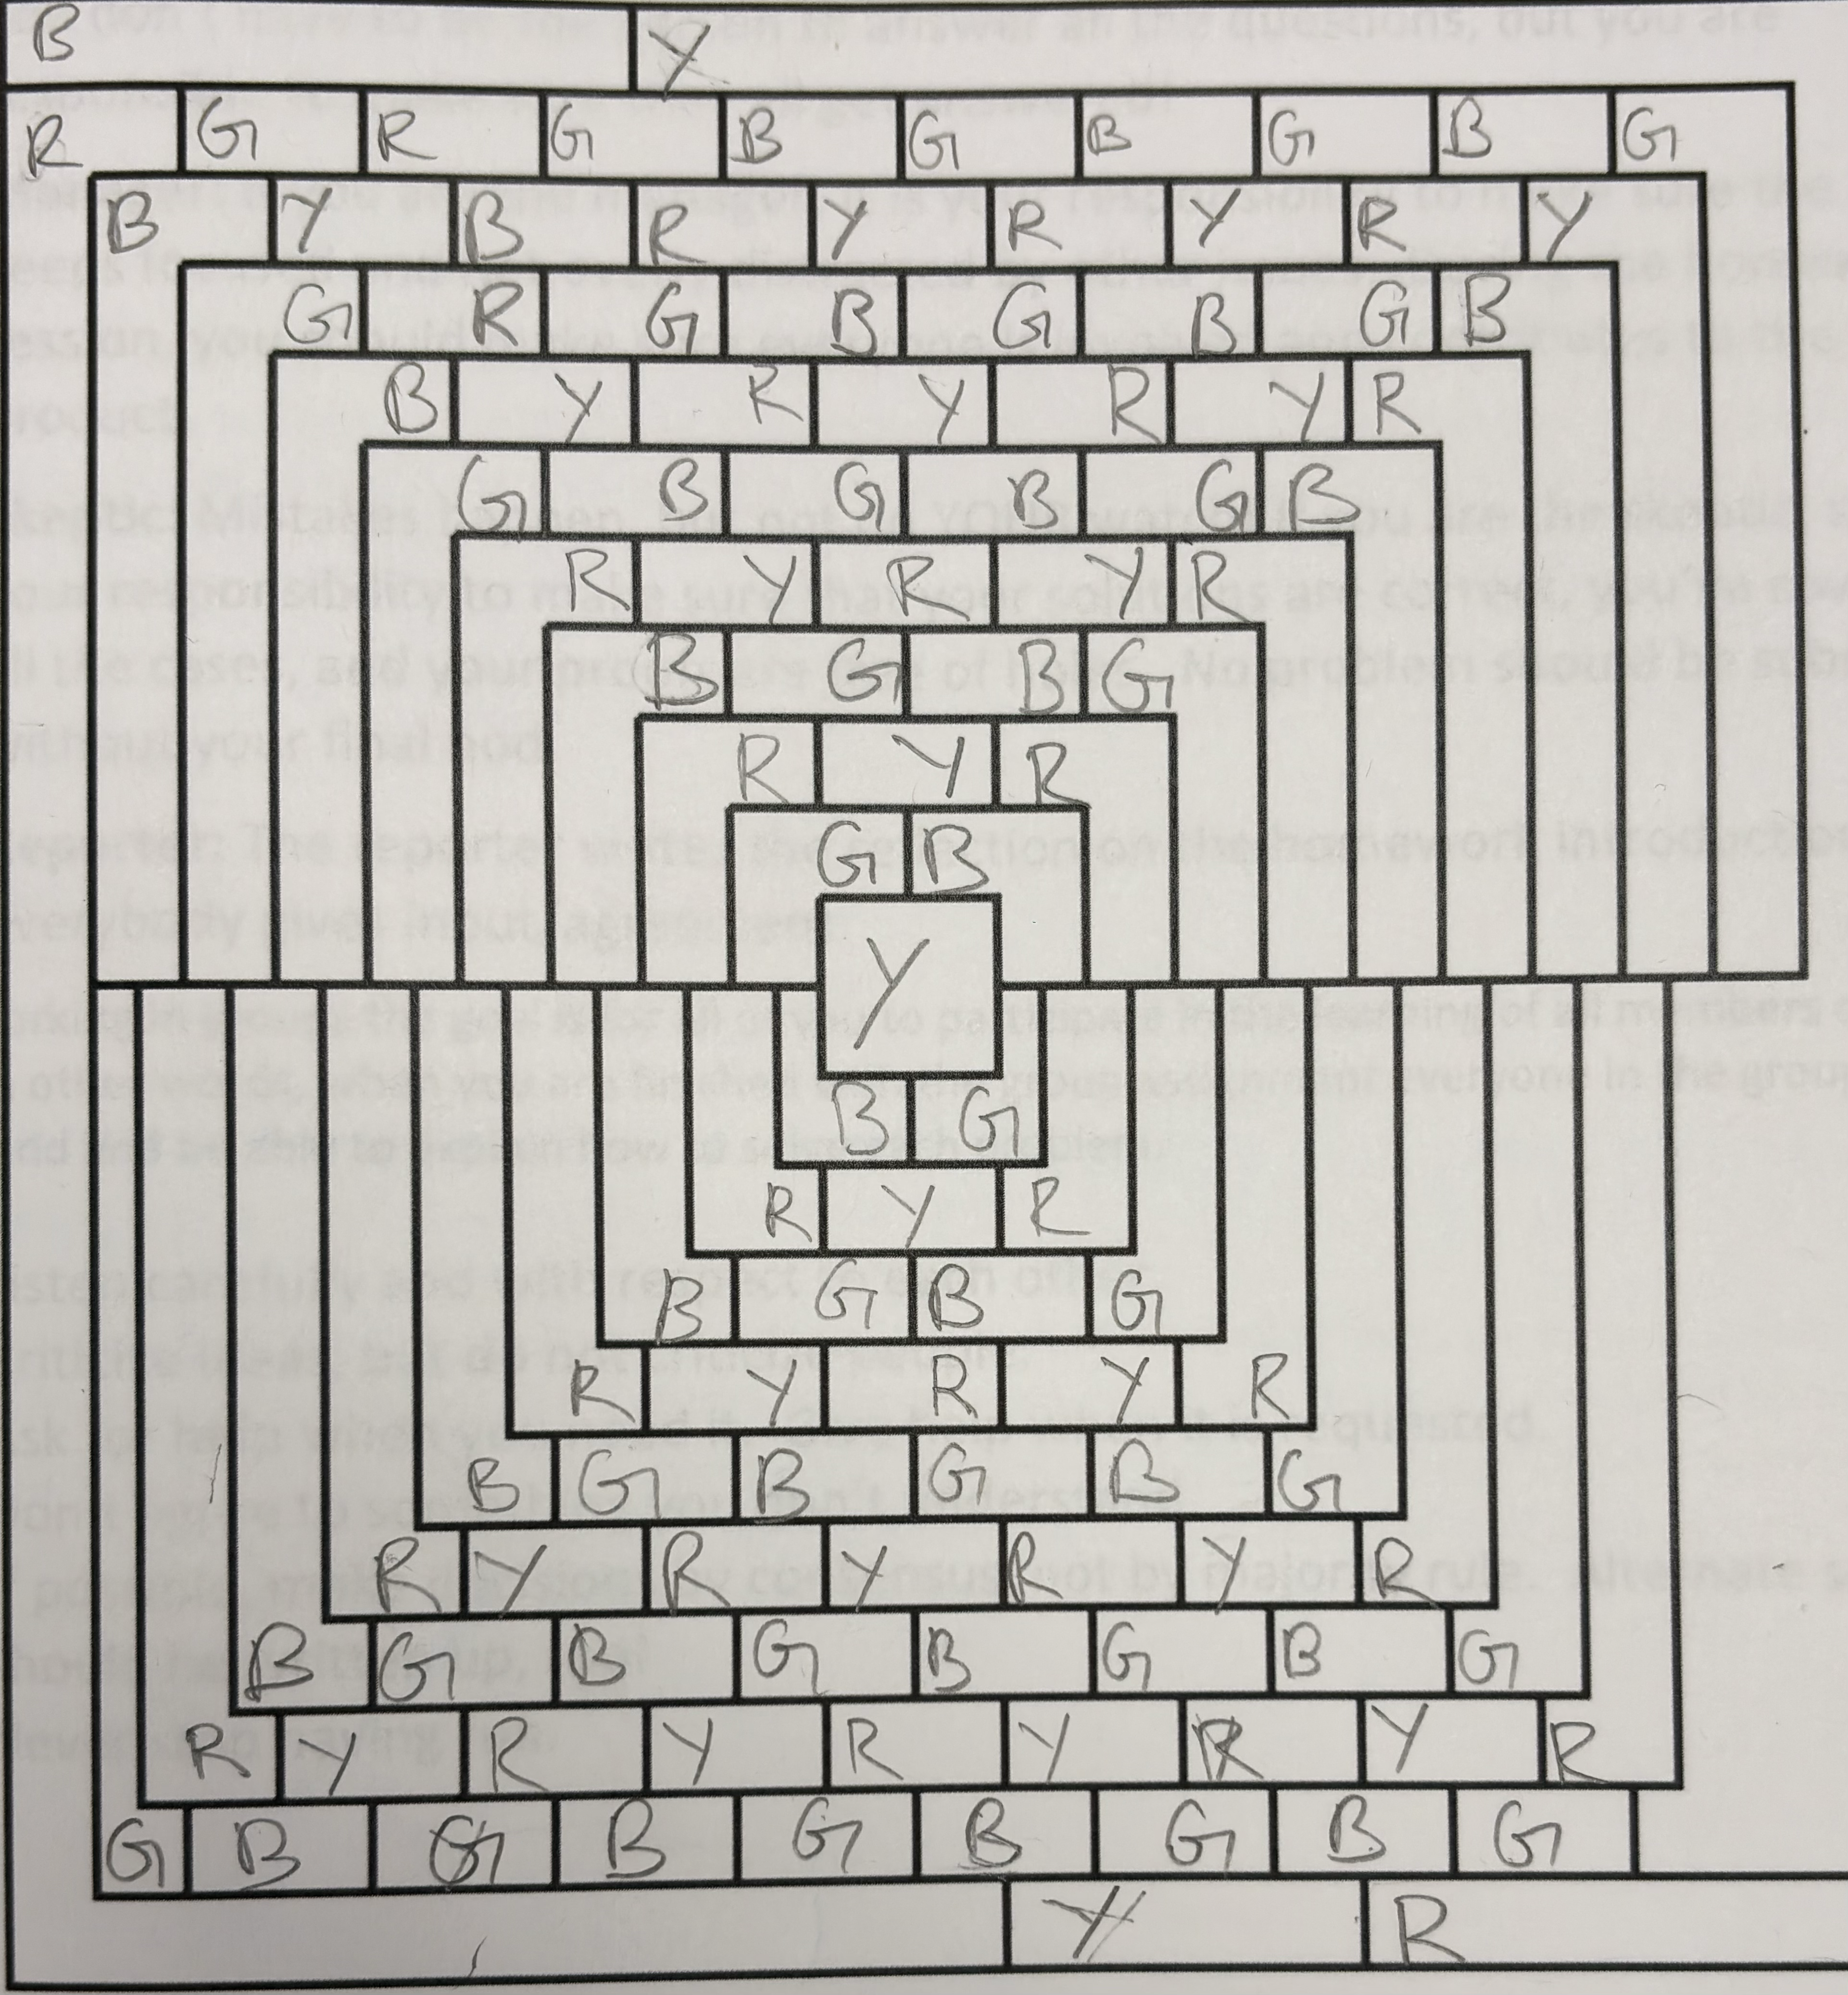
\includegraphics[width=0.25\linewidth]{assets/graphy graphy.png}};
        \end{graphfig}
    \end{solution} \color{red}Look at the tall regions; you have a ton of the same color touching each other! \color{black}
    %yeah, we showed that. 
        \item Back to cutthroat, classify the path graphs up to $p_{14}$, or further. 
    \begin{solution}
        We have confirmed that the known possible $P$-game values possible for $p_n$ is $n=1,4,12,20,30,46,72,98,124,150,176,314,408$. We have run a computer simulation with the given system. A naive solution stalls at $n=55$, while the grundy solution continues without fault and is only limited by computational availability. Our simulations have proven that 408 is the largest $n$ until 1M, and  Caines et al. [1999](chain referenced from Guy and Nowakowski, "Unsolved Problems," 465.) has verified this value up to 50M. The existence of the 14th $p$-number is an unsolved problem. \color{red}Nice work!\color{black}
    \end{solution}
    \item Prove that every non-empty graph's chromatic polynomial has at least one coefficient that is negative. 
    \begin{proof}
        We prove this using two inductive steps. First, we induct on the order $n,$ and second we induct on the size such that for all graphs of smaller order and size $n-1$ there exists a nonzero coefficient of $k^{n-1}$. \color{red}You want the leading coefficient to be exactly one, not just nonzero, for this proof!\color{black} The base case is the empty graph. Now we note that by the equation we found earlier, stating:
        $$
        p_k(G) = p_k(G-e) - p_k(G*e),
        $$

        We have $p_k(G*e)$ containing a $k^{n-1}$ as it has one lower node and size satisfying our inductive assumption. Now we note that $p_k(G-e)$ maintains the same amount of nodes but one smaller size, but the extra node adds another factor of $k$ to contain a $k^n$ factor, which is unaffected by $p_k(G*e).$ Thus, $p_k(G)$ contains a $k^n$ term. As $k^n$ is the maximum value for $p_k(G)$ (the $p_k$ value for an empty graph with $n$ nodes), we must have some term that is subtracted to obtain a smaller value.\color{red}This proof mostly works! You should mention why this maximum is only attained for the empty graph, but it's reasonably clear.\color{black}

        %Note: Sorry this proof basically sucks, it was written in like 5 minutes..

    \end{proof}
    \item Prove that if a graph is color-critical with chromatic number $k$, the minimum degree of the graph has to be equal to $k-1$.
    \item Prove that the graph below is color critical. 
    \begin{graphfig}{NUM}
        \node [v] (a1) at (0, 1){};
        \node [v] (a2) at (0, -1){};
        \node [v] (a3) at (1, 0){};
        \node [v] (a4) at (2, 0){};
        \node [v] (a5) at (3, 1){};
        \node [v] (a6) at (3, -1){};
        \node [v] (a7) at (5, 0){};
        \node [v] (a8) at (6, 1){};
        \node [v] (a9) at (6, -1){};
        \node [v] (a10) at (6, 3){};
        \node [v] (a11) at (6, -3){};
        \node [v] (a12) at (7, 0.5){};
        \node [v] (a13) at (7, -0.5){};
        \node [v] (a14) at (8, 1){};
        \node [v] (a15) at (8, -1){};
        \node [v] (a16) at (10, 0){};
        \draw (a1)--(a2)--(a3)--(a1);
        \draw (a3)--(a4)--(a5)--(a6)--(a4);
        \draw (a5)--(a10) (a6)--(a11) (a1)--(a10) (a2)--(a11) (a7)--(a10) (a7)--(a11) (a7)--(a8)--(a12)--(a13)--(a9)--(a7) (a8)--(a14) (a9)--(a15) (a12)--(a14) (a13)--(a15) (a10)--(a16) (a11)--(a16) (a14)--(a16) (a15)--(a16);
    \end{graphfig}
    \begin{proof}
        We aim to color using only three colors.
        Assuming the color of the middle point is 1, the topmost and bottommost points cannot be 1.
            
        \begin{graphfig}{NUM}
            \node [v] (a1) at (0, 1){};
            \node [v] (a2) at (0, -1){};
            \node [v] (a3) at (1, 0){};
            \node [v] (a4) at (2, 0){};
            \node [v] (a5) at (3, 1){};
            \node [v] (a6) at (3, -1){};
            \node [v] (a7) at (5, 0){};
            \node [v] (a8) at (6, 3){};
            \node [v] (a9) at (6, -3){};
            \draw (a1)--(a2)--(a3)--(a1);
            \draw (a3)--(a4)--(a5)--(a6)--(a4) (a1)--(a8) (a2)--(a9) (a8)--(a7)--(a9) (a5)--(a8) (a6)--(a9);
        \end{graphfig}
        Case 1(Graph 10): If the topmost and bottommost points share the same color (e.g., 2), the top-left point becomes 1 and the bottom-left point becomes 3. Consequently, the middle-left point would have to be 2, making it impossible to fill all three points on the left side (top, middle, and bottom).
            
        \begin{graphfig}{NUM}
            \node [v] (a7) at (5, 0){};
            \node [v] (a8) at (6, 1){};
            \node [v] (a9) at (6, -1){};
            \node [v] (a10) at (6, 3){};
            \node [v] (a11) at (6, -3){};
            \node [v] (a12) at (7, 0.5){};
            \node [v] (a13) at (7, -0.5){};
            \node [v] (a14) at (8, 1){};
            \node [v] (a15) at (8, -1){};
            \node [v] (a16) at (10, 0){};
            \draw (a7)--(a10) (a7)--(a11) (a7)--(a8)--(a12)--(a13)--(a9)--(a7) (a8)--(a14) (a9)--(a15) (a12)--(a14) (a13)--(a15) (a10)--(a16) (a11)--(a16) (a14)--(a16) (a15)--(a16);
        \end{graphfig}
        Case 2(Graph 11): If the topmost and bottommost points have different colors (top: 2, bottom: 3), the rightmost point becomes 1. Then, the upper-middle-right point must be 2, and the top-right point must be 3. Thus, the upper point among the middle-right positions becomes 1; following the same logic, the lower point among the middle-right positions must also be 1. This leads to a contradiction.
        Therefore, it is impossible to color using only three colors. \color{red}Here you want to show this is 3-colorable after removing any vertex, not just that the original graph has chromatic number 4!\color{black}
    \end{proof}
    \item Find the chromatic polynomial of the graph below.
    \begin{graphfig}{NUM}
        \node [v] (a1) at (0, 1){};
        \node [v] (a2) at (0, 0){};
        \node [v] (a3) at (1, 0){};
        \node [v] (a4) at (1, 1){};
        \node [v] (a5) at (2, 1){};
        \node [v] (a6) at (2, 0){};
        \node [v] (a7) at (3, 0){};
        \node [v] (a8) at (3, 1){};
        \draw (a1)--(a2)--(a3)--(a4)--(a5)--(a6)--(a7)--(a8) (a1)--(a4) (a5)--(a8);
    \end{graphfig}
    \begin{solution}
        If we remove one edge from graph 9, it will look like graph 11. Additionally if we merge 2 vertices together it will look like graph 10. Since $p_k(graph10) = k(k-1)^2(k^2-3k+3)^2$, $p_k(graph11)=k^2(k-1)^2(k^2-3k+3)^2$, $p_k(graph 9) = p_k(graph 11) p_k(graph10)=k(k-1)^3(k^2-3K+3)^2$\color{red}This is right, but you should briefly explain these chromatic polynomials. Also consider naming the graphs, maybe something like $G,G_*, G_-.$ And inline math mode may not be best here.\color{black}
    \end{solution}
    \begin{graphfig}{NUM}
        \node [v] (a1) at (0, 1){};
        \node [v] (a2) at (0, 0){};
        \node [v] (a3) at (0.5, 0){};
        \node [v] (a4) at (1, 1){};
        \node [v] (a5) at (1.5, 0){};
        \node [v] (a6) at (2, 0){};
        \node [v] (a7) at (2, 1){};
        \draw (a1)--(a2)--(a3)--(a4) (a4)--(a5)--(a6)--(a7) (a1)--(a4) (a4)--(a7);
    \end{graphfig}
    \begin{graphfig}{NUM}
        \node [v] (a1) at (0, 1){};
        \node [v] (a2) at (0, 0){};
        \node [v] (a3) at (1, 0){};
        \node [v] (a4) at (1, 1){};
        \node [v] (a5) at (2, 1){};
        \node [v] (a6) at (2, 0){};
        \node [v] (a7) at (3, 0){};
        \node [v] (a8) at (3, 1){};
        \draw (a1)--(a2)--(a3)--(a4) (a5)--(a6)--(a7)--(a8) (a1)--(a4) (a5)--(a8);
    \end{graphfig}
    \item \color{blue}\textit{UNSOLVED} \color{black} Is it true that, if, for all \textit{adjacent} vertices $a$ and $b$, $\chi(G-\{a,b\})=\chi(G)-2$ has to be complete? 
    \item \color{blue}\textit{UNSOLVED} \color{black} \textit{Erdos : The Dense Triangle Free Conjecture}. If $G$ is a triangle-free graph whose minimum degree exceeds $1/3$ of the number of vertices, the $G$ can be colored in four colors. Can you prove it or find a counterexample? 
    \item \color{blue}\textit{UNSOLVED} \color{black} Are there more than 7 unipancyclic graphs? 
\end{enumerate}
\color{docshaw}
Nicely done overall. Take Z's comments seriously, and be proud that you did a great assignment.
\end{document}